\section{Faster Path-ORAM with B-Trees}

When a client stores data in a Path-ORAM\cite{ShiCCS13}, it needs to 
maintain a position map. The position map stores a leaf node of 
the Path-ORAM pertaining to each data that is 
stored in the Path-ORAM. 
The data is stored in one of the nodes in 
the path from the root to that leaf node.
The position map can be stored at the client, 
which increases client storage. Or, it can be recursively
stored in Path-ORAMs at the server, which
increases the number of communication rounds to the server.



A Path-ORAM can be instantiated with an AVL-tree. 
An AVL Tree is a self balancing binary search tree.
There is an advantage and a disadvantage 
of instantiating an ORAM with an AVL tree. 
The advantage is that the client can get rid of the position map.
Because, AVL trees are binary search trees,
the left subtree of a node contains only nodes 
with keys lesser than the node’s key, and 
the right subtree of a node contains only nodes
with keys greater than or equal to the node’s key,
(obviously left and right subtrees are 
binary search trees as well). When a Path-ORAM 
is instantiated with an AVL tree,
every AVL tree node (which is basically a Path-ORAM node) 
stores the address of its left and right children (see Figure \ref{fig:pathAVL}).
Because of this reason, the client does not need to store the position 
map anymore, instead it can only store
the leaf position pertaining to the root of the AVL-tree.


\begin{figure}[h]
	\centering
	\includegraphics[width=0.45\textwidth]{chapters/iodse/figures/omap.pdf}
	\vspace{-.4cm}
	\caption[Sample AVL Tree and its Path-ORAM]{Sample AVL Tree and its Path-ORAM~\cite{wang2014oblivious, Mitra}.}
	\label{fig:pathAVL}
	%	\vspace{-.6cm}
\end{figure}


To read/write to a node in the AVL-tree one needs to access a whole path of the AVL-tree, in worst case. 
Accessing each AVL node will incur accessing
one Path-ORAM path i.e. $\log N$ Path-ORAM nodes (assuming the Path-ORAM is setup with $N$ elements). In worst case an 
AVL tree of $N$ nodes have height $1.45 \cdot \log N$ \cite{avlheight}.
This means, in worst case it needs to read $1.45 \cdot \log N$ AVL tree nodes.

$$h_{max}^A= 3 \cdot 1.45 \cdot \log_2 N = 4.35 \cdot \log_2 N$$

For inserts and deletes it can be upto $3\cdot 1.45 \cdot \log N$ nodes, because of the rotations in the tree.
If the client wants to hide the operation type, 
i.e. if the client wants to hide if its a read or a write 
then every time a total of 
$\log N \cdot 3\cdot 1.45 \cdot \log N= 4.35 \log^2 N$ 
Path-ORAM nodes need to be fetched. 

My idea is to instantiate Path-ORAM with B-tree instead of 
an AVL tree. 
A B-tree is a self balancing search tree that 
allows a node in the tree to have more than two children
and more than one key. We say a B-tree is of degree $d$, if
each node of the B-tree has \textbf{at most} $d$ children. 
Which means each node has at most $d-1$ keys (see Figure \ref{fig:btree}). 
A B-tree node always must be \textbf{at least} half full (except the root node).
This means each node's degree should be at least $t=\ceil{\frac{d}{2}}$.
The maximum height ($h_{max}^B$) of a B-tree is computed when every node is half full\cite{btree},
i.e. when a B-tree that can store $N$ nodes actually stores $\ceil{\frac{N}{2}}$ nodes.

$$h_{max}^B = \log_t \frac{N}{2}$$

\begin{figure}[h]
%\begin{mdframed}
\centering
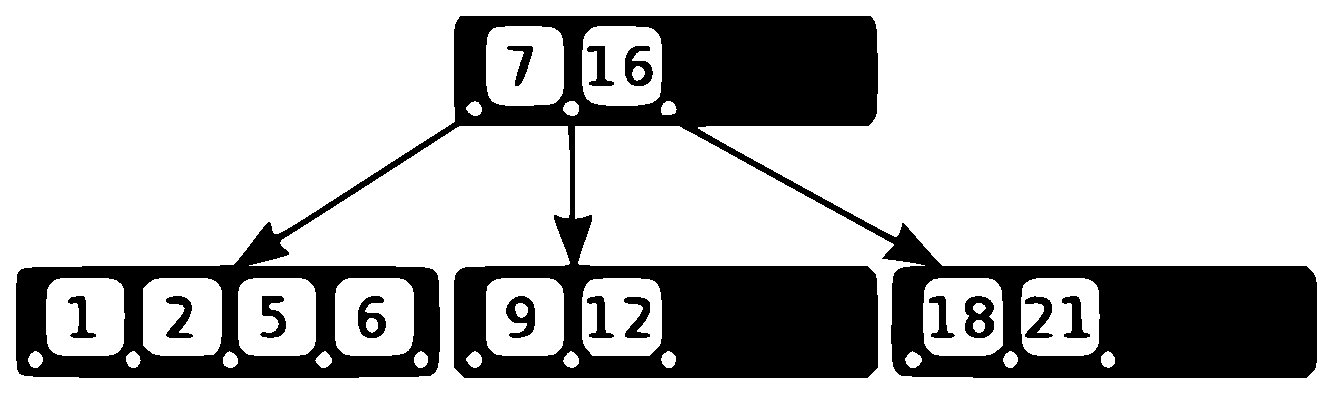
\includegraphics[width=0.7\textwidth]{chapters/iodse/figures/btreepic.eps}
%\end{mdframed}
\caption[B-tree]{B-tree with degree 5}
\label{fig:btree}
\end{figure}

Now we can see that $h_{max}^A > h_{max}^B$ for any B-tree with degree greater than 2. My starting point was to implement B-Tree Path-ORAM and compare its search time with AVL tree Path-ORAM. Figure \ref{fig:avl-btree}
shows search time for a B-tree Path-ORAM vs AVL-tree Path-ORAM for 
different values of $t$ ($2 \leq t \leq 8$). 
The x-axis is the result size, and the y-axis is the search time 
in miliseconds. The experiment was done on a very small dataset
of 200MB, with ~700 searchable keywords. But the results of this
experiment is enough of a motivation to 
proceed further with B-trees. The search time 
for the B-tree (red, yellow and green plots) are better 
than that of AVL-tree (the blue plot). 
The plot for $t=8$ is worse than $t=4$ because 
the amount of data read for $t=8$ becomes huge.
In this case, for each node it reads 8 times more data.
So, there is always 
a trade-off between number of Path-ORAM nodes fetched (i.e. 
the number of times the Path-ORAM is accessed) versus amount of data 
read per node.

\begin{figure}
	\centering
	\includegraphics[width=0.7\textwidth]{chapters/iodse/figures/avl-btree.pdf}
	\vspace{-.4cm}
	\caption[Search time of AVL-tree Path-ORAM vs B-tree Path-ORAM]{Search time of AVL-tree Path-ORAM vs B-tree Path-ORAM (with degrees $d =2t=$ 4,8 and 16)}
	\label{fig:avl-btree}
	%	\vspace{-.6cm}
\end{figure}

\subsection{B-tree Path-ORAM for files.}

B-trees are known to be well suited for operations 
with large data on file systems and databases. 
Hence B-tree Path-ORAM is a good choice for storing files.


